\chapter[Preprocessing of time series]{Compression for a better classification with Dynamic Time Warping}

\begin{abstract}
 Dynamic Time Warping (DTW) is a time series alignment algorithm that is often used because it
 considers that it exits small distortions between time series during their alignment.  However, DTW
 sometimes produces pathological alignments that occur when, during the comparison of two time series
 X and Y, one data point of the time series X is compared to a large subsequence of data points of Y.
 In this paper, we demonstrate that to compress time series using Piecewise Aggregate Approximation
 (PAA) is a simple strategy that greatly increases the quality of the alignment with DTW this is
 particularly true for synthetic data sets.      
 \end{abstract}

\section{Introduction}

Time series databases are often large and several transformations have been
introduced in order to represent them in a more compact way. One of these transformations is
Piecewise Aggregate Approximation (PAA) \cite{keogh2001dimensionality}, which consists in dividing a
time series into several segments of fixed length and replacing the data points of each segment with
their averages. Due to its simplicity and low computational time, PAA has been widely used as a
basic primitive by other temporal data mining algorithms such as \cite{lin2003symbolic,
sun2014improvement, lkhagva2006extended}, in order  
\begin{itemize}
  \item To construct symbolic representations of time
series; \cite{camerra2010isax, ulanova2015scalable}.
  \item To construct an index for time series; \cite{zhao2016shapedtw,
keogh2000scaling, Kate2016}. Indeed, PAA allows queries which are shorter than length for which the
index was built, this very desirable feature is impossible in Discrete Fourier Transform, Singular
Value Decomposition and Discrete Wavelet Transform.
\item To classify time series.
\end{itemize}


\subsection{Why the use of PAA can improve alignment with Dynamic Time Warping}

An important task is time series comparison  that
can be done in two main ways.
Either the comparison method  considers that there is no time distortion as in Euclidian distance
(ED), or it considers that  some small time distortions  exist between time axis of time series as
in Dynamic Time Warping alignment algorithm (DTW)
\cite{ZhangTangDuan2015}. Since time distortion often exists between time series, DTW often has
better results than the ED \cite{UCRArchive}. An exhaustive comparison of time series algorithms
\cite{Bagnall} shows that DTW is among the efficient techniques to be used. However, DTW has two major
drawbacks:
 the comparison of two time series under DTW is time-consuming
\cite{Rakthanmanon2012} and  DTW
sometimes produces pathological alignments \cite{KeoghPazzani2001}. A
pathological alignment occurs when, during the comparison of two time  series $X$
and $Y$, one datapoint of the time series $X$ is compared to a large subsequence
of datapoints of $Y$.  A pathological alignment causes a wrong comparison.


 Three categories of methods are used to avoid pathological alignments with DTW:

\begin{itemize}
  \item The first one adds constraints to DTW \cite{RatanamahatanaKeogh2004, YuYuHuLiuWu2011, candan2012sdtw, SakoeChiba1978, jeong2011weighted}.
  The main idea here is to limit the length of the subsequence of a time series
  that can be compared to a single datapoint of another time series.
  
  \item The second one suggests skipping datapoints that
  produce pathological alignment during the comparison of two time series \cite{longin2005elastic, itakura1975minimum, MyersRabinerRosenberg1980}.
  \item The third one proposes to replace the datapoints of time
  series with a high-level abstraction that captures the local behavior of those
  time series. A high-level abstraction can be a histogram of values that
  captures the repartition of time series datapoints in space \cite{ZhangTangDuan2015} or a 
  feature that captures the local  properties of time series, such as the trend with Derivative DTW
  (DDTW) \cite{KeoghPazzani2001}.
\end{itemize}
Another simple but yet interesting way to capture local properties of time series is to consider
mean of segments of the time series as PAA does. Indeed, the use of the mean reduces the harmful
effects of singularities contained in the data and thus allows to avoid the pathological
alignments.  However, one major challenge with PAA is the choice of the number of segments to
consider especially with long time series.


\subsection{The problem of choosing a suitable segment number for PAA}

If the number of segments considered with PAA is too small, the resulted
representation  is compact, but it contains less information. On the other side, if the number of
segments is too large, the obtained representation  is less compact and more prone to the noise
contained in the original time series (Fig. \ref{relation_nb_acc}). Our idea is that a number of
segments for PAA will be considered as good if it allows obtaining a compact representation of the
time series, and also if it preserves the quality of the alignment of time series. So when
considering classification task, one of the best classification algorithm to use for
evaluating the quality of time series alignment is one nearest neighbor (1NN).   
Indeed, its classification error directly depends on time series alignment, since 1NN has no other
parameters \cite{wang2013experimental}.


\begin{figure}[h]
\center
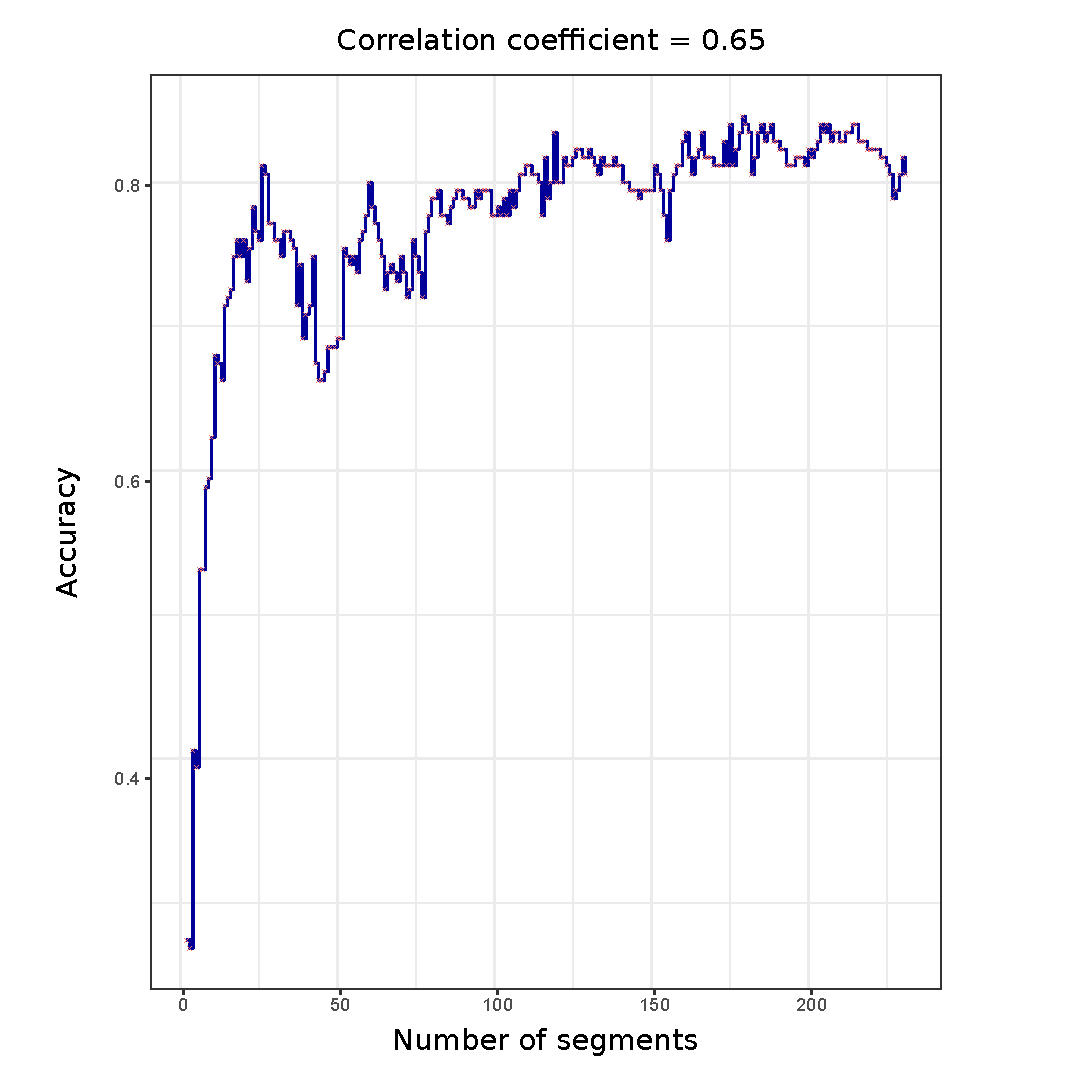
\includegraphics[scale = 0.4]{images/effets_de_n_sur_accuracy}
\caption{Relation between Accuracy and the number of segment on FISH dataset. The accuracy is computed from the algorithm one nearest neighbor associated with PDTW. When the number of segments
considered is very small, there is a loss of information and the accuracy is reduced. However, considering all the points in the time series, we also do not obtain maximum accuracy due to the presence of noise or singularities \cite{KeoghPazzani2001}  in the data. }
\label{relation_nb_acc}
\end{figure}

\subsection{Summary of Contributions}

In this paper, 
\begin{itemize}
\item We define the problem of preprocessing time series with PAA for a better classification with
DTW.
\item We propose a parameter free heuristic for aligning piecewise aggregate time series with DTW, which approximates the optimal value of the number of segments to be considered with PAA. 
\item  We make our source code and all our results available to allow the reproducibility of
our experiments.
work.
\end{itemize}

The rest of the paper is organized as follow: In Section
\ref{sec:1} we recall the definitions and background. Section \ref{sec:2} explains our approach.
Section \ref{sec:3} presents experimental results and comparisons to others methods. Section
\ref{sec:4} offers conclusions and venues for future work.   


\section{Background and related work}
\label{sec:1}
Let's recall some definitions.

\begin{definition}:  A \textbf{time series}
$X=x_{1},\cdots,x_{n}$ is a sequence of numerical values representing the evolution of a specific quantity over time. $x_{n}$ is the most recent value.
\end{definition}

\begin{definition}:
A segment  $X_{i}$ of length  $l$ of the time series $X$ of length $n$
$(l<n)$ is a sequence constituted by $l$ \hyphenation{conse-cutive} variables of $X$ starting at the position $i$ and ending at the position $i+l-1$.
We have: $X_{i}=x_{i},x_{i+1},...,x_{i+l-1}$
\end{definition}

\begin{definition}:
The arithmetic average of the data points of a segment  $X_{i}$ of length
$l$ is noted $\bar{X}_{i}$ and is defined by:
\begin{eqnarray}
\bar{X}_{i}=\frac{1}{l}\sum_{j=0}^{l-1}x_{i+j}
\end{eqnarray}

\end{definition}

\begin{definition}:
Let $T$ be the set of time series. The Piecewise Aggregate Approximation (PAA) is defined as follows:

\begin{eqnarray}
\begin{array}{ccc}
 PAA: T\times\mathbb{N^{*}}\rightarrow T\\
\\
(X,N)\mapsto PAA(X,N) & = &
 \begin{cases}
 \begin{array}{c}
\bar{X}_{1},\cdots,\bar{X}_{N}\:if\:N<|X|\\
X\:otherwise
\end{array}
\end{cases}
\end{array}
\end{eqnarray}

\end{definition} 

\begin{definition}:
Let $d\subseteq T$ be a subset of time series,
$N\in\mathbb{N}^{*},\:PAAset(d,N)=\{PAA(X,N),\:\forall X\in d\}$
\end{definition}

\subsection{Dynamic Time Warping algorithm.}
DTW \cite{sakoe1978dynamic} is an algorithm of time series alignment
algorithm that  performs a non-linear alignment while
minimizing the distance between two time series. To align two time series : 
$X=x_{1},x_{2},\cdots,x_{n};\,
Y=y_{1},y_{2},\cdots,y_{m},$ the algorithm constructs an  $n\times m$  matrix where the cell $(i,
j)$ of the matrix corresponds to the squared distance $(x_{i}-y_{j})^{2}$ between $x_{i}$
and $y_{j}$. To find the best alignment between two time series, DTW constructs the path that minimizes the sum of squared distances. This path, noted
$W = w_1, w_2, \ldots, w_k, \ldots, w_K,$ must respect the following constraints:
\begin{itemize}
  \item Boundary constraint: $w_1 = (1, 1)$ and  $w_K = (n, m)$
  \item Monotonicity constraint: given $w_k = (i, j)$ and :  $w_{k + 1} =
  (i',j')$ then : $i \leq i'$ and $j \leq j'$
 \item Continuity constraint: given $w_k = (i, j)$ and :   $w_{k + 1} = (i', j')$
 then : $i' \leq i + 1$ and : $j' \leq j + 1$
\end{itemize}
The warping path is computed by  an algorithm based on the dynamic
programming paradigm that solves the following recurrence:
\begin{eqnarray}
\gamma(i,j)=d(x_{i},y_{j})+min\{\gamma(i-1, j-1),\gamma(i-1, j),\gamma(i, j-1)\},
\end{eqnarray}


where $d(x_{i},y_{j})$ is the squared distance contained in the cell $(i, j)$ and $\gamma(i, j)$ is the cumulative distance at the position $(i, j)$ that is computed by the sum of the squared distance at the position $(i, j)$ and the minimal cumulative distance of its three adjacent cells.


\subsection{Piecewise Dynamic Time Warping}

Piecewise Dynamic Time Warping Algorithm (PDTW) \cite{keogh2000scaling} is the DTW algorithm applied on Piecewise Aggregate time series \cite{Keogh2001}. Let $N\in\mathbb{N^{*}}$, $X$ and $Y$ be two time series.
\begin{eqnarray}
PDTW(X, Y, N) = DTW(PAA(X, N), PAA(Y, N)).
\end{eqnarray}


\section[Heuristic]{Heuristic search of the number of segments}
\label{sec:2}
\subsection{Problem definition.}

\begin{definition}
Let $D = \{d_i\}$ be a set of datasets composed of time series and $X \in d_i$ be a time series of
the dataset $d_i$; we note $|X| = n$ the length of the time series $X$. Let $N\in\mathbb{N}^{*} and \,N \leq n$, $1NNPDTW( d_i, N)$  is the
classification error of 1-NN with PDTW using $N$ segments on $d_i$.
\end{definition}


Our goal is to find a number of segments $N
\in \{1 \ldots n \}$ such that
\[
1NNPDTW(d_{i},N)=\underset{1\leq\alpha\leq n}{min}\{1NNPDTW(d_i,\alpha)\}.
\]


The simplest way to find the value for the number of segments that minimized the
classification error is to test all the possible values.  Obviously, this method is time-consuming as we have to test $n$ values to find the one
that has the minimal classification error. The time complexity of this process is :
\[
O((\frac{|trainingset|}{2})^{2} \times \underset{N\in C}{\sum}{\displaystyle
N^{2}}),\, |C|=n,
\]

where $C$ is the set of values for the number of segments.

To reduce the time of the search, the FDTW proposes to look for the
number of segments with the minimal classification error without testing all the possible values.

\subsection{ Greedy Randomized Adaptive Search Procedures}
The Greedy Randomized Adaptive Search Procedures (GRASP) is a multi-start, or iterative metaheuristic proposed by Feo and Resende
(1995) \cite{feo1995greedy}, in which each iteration consists of two phases:
firstly a new solution is constructed by a greedy randomized
procedure and  then is improved using a local search procedure.


The greediness criterion establishes that elements with the best quality are
 added to a restricted candidate list and chosen at random when
building up the solution. The candidates obtained by greedy algorithms are not
necessarily optimal. So, those candidates are  used as initial solutions
to be explored by local search. The heuristic that we proposed is build upon
GRASP and strengthened with an inclusion of specific global search component.


\subsection{Parameter free heuristic}

The idea of our heuristic is the following:

\paragraph{1.} We choose $N_{c}$ candidates distributed in the space of possible values
to ensure that we are going to have small, medium and large values as
candidates. The candidates values are: $n,\,n-\left\lfloor
\frac{n}{N_{c}}\right\rfloor ,\,n-2\times\left\lfloor \frac{n}{N_{c}}\right\rfloor
,\,...,\,n-N_{c}\times\left\lfloor \frac{n}{N_{c}}\right\rfloor $. For instance, if the length of
time series is $n = 12$ and the number of candidates is $N_c = 4$, we are going to select the
candidates 12, 9, 6, 3.
\begin{center}

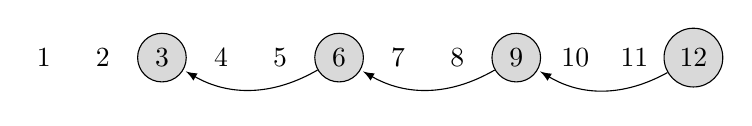
\begin{tikzpicture}[shorten >=1pt,->]
\node (1) at (1,1) {1};
\node (2) at (1.75,1) {2};
\node[draw,circle,fill=gray!30] (3) at (2.5,1) {3};
\node (4) at (3.25,1) {4};
\node (5) at (4,1) {5};
\node[draw,circle,fill=gray!30] (6) at (4.75,1) {6};
\node (7) at (5.5,1) {7};
\node (8) at (6.25,1) {8};
\node[draw,circle,fill=gray!30] (9) at (7,1) {9};
\node (10) at (7.75,1) {10};
\node (11) at (8.5,1) {11};
\node[draw,circle,fill=gray!30] (12) at (9.25,1) {12};

\draw[->,>=latex] (12) to[bend left] (9);
\draw[->,>=latex] (9) to[bend left] (6);
\draw[->,>=latex] (6) to[bend left] (3);

\end{tikzpicture}
\end{center}


\paragraph{2.} We evaluate the classification error with $1NNPDTW$ for each chosen candidate, and we
select the candidate that has the minimal classification error: it is the best candidate.
In our example, we may suppose that we get the minimal value with the candidate 6 : it is thus the
best candidate at this step.

\begin{center}

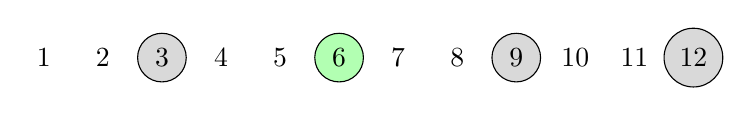
\begin{tikzpicture}[shorten >=1pt,->]

\node (1) at (1,1) {1};
\node (2) at (1.75,1) {2};
\node[draw,circle,fill=gray!30] (3) at (2.5,1) {3};
\node (4) at (3.25,1) {4};
\node (5) at (4,1) {5};
\node[draw,circle,fill=green!30] (6) at (4.75,1) {6};
\node (7) at (5.5,1) {7};
\node (8) at (6.25,1) {8};
\node[draw,circle,fill=gray!30] (9) at (7,1) {9};
\node (10) at (7.75,1) {10};
\node (11) at (8.5,1) {11};
\node[draw,circle,fill=gray!30] (12) at (9.25,1) {12};

\end{tikzpicture}

\end{center}

\paragraph{3.} We respectively look between the predecessor (i.e., 3 here) and successor (i.e., 9
here) of the best candidate for a number of segments with a lower classification error : this number
of segments corresponds to a local minimum.
In our example, we are going to test values 4, 5, 7 and 8 to see if there is a local minimum.

\begin{center}

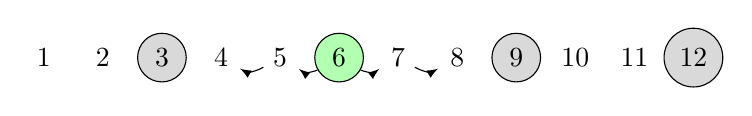
\begin{tikzpicture}[shorten >=1pt,->]

\node (1) at (1,1) {1};
\node (2) at (1.75,1) {2};
\node[draw,circle,fill=gray!30] (3) at (2.5,1) {3};
\node (4) at (3.25,1) {4};
\node (5) at (4,1) {5};
\node[draw,circle,fill=green!30] (6) at (4.75,1) {6};
\node (7) at (5.5,1) {7};
\node (8) at (6.25,1) {8};
\node[draw,circle,fill=gray!30] (9) at (7,1) {9};
\node (10) at (7.75,1) {10};
\node (11) at (8.5,1) {11};
\node[draw,circle,fill=gray!30] (12) at (9.25,1) {12};

\draw[->,>=latex] (6) to[bend left] (5);
\draw[->,>=latex] (5) to[bend left] (4);
\draw[->,>=latex] (6) to[bend right] (7);
\draw[->,>=latex] (7) to[bend right] (8);

\end{tikzpicture}

\end{center}


\paragraph{4.} We restart at step one while choosing
different candidates during each iteration to ensure that we return a good
local minimum. We fix the number of iterations to $k \leq \left\lfloor log(n)\right\rfloor $. At each iteration, the first candidate is $n-(number \_ of \_ iteration \,-\, 1)$.

\paragraph{}In short, in the worst case, we test the first $N_{c}$ candidates to find the best one.
Then, we test $\frac{2n}{N_{c}}$ other candidates to find the local minimum.
We finally perform $nb(N_{c})\, =\, N_{c}\, +\, \frac{2n}{N_{c}}$ tests. The number of tests
 to be performed is a function of the number of candidates. Hence, how many
candidates should we consider to reduce the number of tests? The first
derivative of $nb$ function  vanishes when $N_{c}=\sqrt{2n}$ and its second derivative is
positive; so the minimal number of tests is obtained when the number of candidates is : 
$N_{c}=\sqrt{2n}$.

\paragraph{Lemma 1.}:
For a given a dataset $d_i$,
$ FDTW(d_{i}) \leq 1NNDTW(d_{i}) $. The quality of the alignment of our heuristic
is better than that of DTW.


\paragraph{Proof}:
 $1NNDTW(d_i) = 1NNPDTW(d_i,n)$. Then, $1NNDTW(d_i)$ is one of the
candidates considered by the heurisitic $FDTW$. Since $FDTW$ returns the
minimal classification error from all candidates, the classification error of
$1NNDTW$ is always greater than or equal to $FDTW$.

\paragraph{} A heuristic does not always give the optimal value. To ensure that
it gives a result not far from the optimal value, one approach is to
 guarantee that the result of the heuristic always lies in an interval with respect to the optimal
value \cite{ibarra1975fast}.

In our case, we are looking for the number of segments that allows a good
alignment of time series. The alignment is good when the classification error
with 1NN is minimal or when the accuracy is maximal.


Let $d_i$ be a dataset:

$acc_{max(d_i)} = 1-\underset{1\leq\alpha\leq n}{min}\{1NNPDTW(di,\alpha)\}$ is the maximal accuracy
for the dataset $d_i$,

$acc_{DTW} = 1 - 1NNDTW(d_i)$ is the accuracy with $d_i$ and 1NNDTW and


$acc_{FDTW}=1 - FDTW(d_i)$ is the accuracy of our heuristic.

To ensure the quality of our heuristic FDTW, wee hypothesized tat $1NNDTW$ is better than
Zero Rule classifier. Zero Rule classifier is a simple classifier that predicts the majority class of test data (if nominal) or average value (if numeric). Zero Rule is often
used as baseline classifier \cite{cuvrin2007meeting}. The minimal value of the
accuracy of Zero Rule is $\frac{1}{c}$ where c is the number of classes of the
dataset.

\paragraph{Proposition 1.}:
For a given dataset $d_i$ that has $c_i$ classes, $c_i\in \mathbb{N}^*,$

$
if \; acc_{DTW} \geq \frac{1}{c_i} \; then \;  \frac{1}{c_i} \times acc_{max}
\leq acc_{FDTW} \leq acc_{max}
$

Proposition 1 shows that when 1NN associated with DTW has a better accuracy than the baseline
classifier Zero Rule, the FDTW heuristic is an approximation.

\begin{flushleft}:
By definition, $ acc_{FDTW} \leq acc_{max}$ 
We look for $\beta \in \mathbb{N}$ such that 
\begin{eqnarray}
\frac{1}{\beta} \times acc_{max} \leq acc_{FDTW} \\
\frac{1}{\beta}\times acc_{max}\leq acc_{FDTW}\Leftrightarrow\frac{acc_{max}}{acc_{FDTW}}\leq \beta \\
However,\quad \frac{acc_{max}}{acc_{FDTW}}\leq\frac{1}{acc_{FDTW}}\quad \\
because\quad acc_{max}\leq1
\\
And,\quad \frac{1}{acc_{FDTW}}\leq\frac{1}{acc_{DTW}} \quad \\
because \quad acc_{DTW}\leq acc_{FDTW}
\\
So,\quad \frac{1}{acc_{DTW}}\leq c_{i} \quad \\
because \quad \frac{1}{c_{i}}\leq
acc_{DTW} \quad by \quad hypothesis
\end{eqnarray}
we take $\beta = c_{i}$.

\end{flushleft}


\section{Experiments and discussion}
\label{sec:3}
\subsection{Datasets}
The performance of FDTW has been evaluated on  84 datasets of the UCR
time series datamining archive \cite{UCRArchive}, which provides a large collection of
datasets that cover various  domains. Each dataset is divided
into a training set and a testing set.

\subsection{Compression}
When it is used with a suitable segments number determined with FDTW, PAA allows compression of the
time series of the \textbf{Coffee}  without loss of information. Although they are more
compact, the obtained time series capture the main variations of the original time series (Fig.
\ref{coffee}).

\begin{figure}
\center
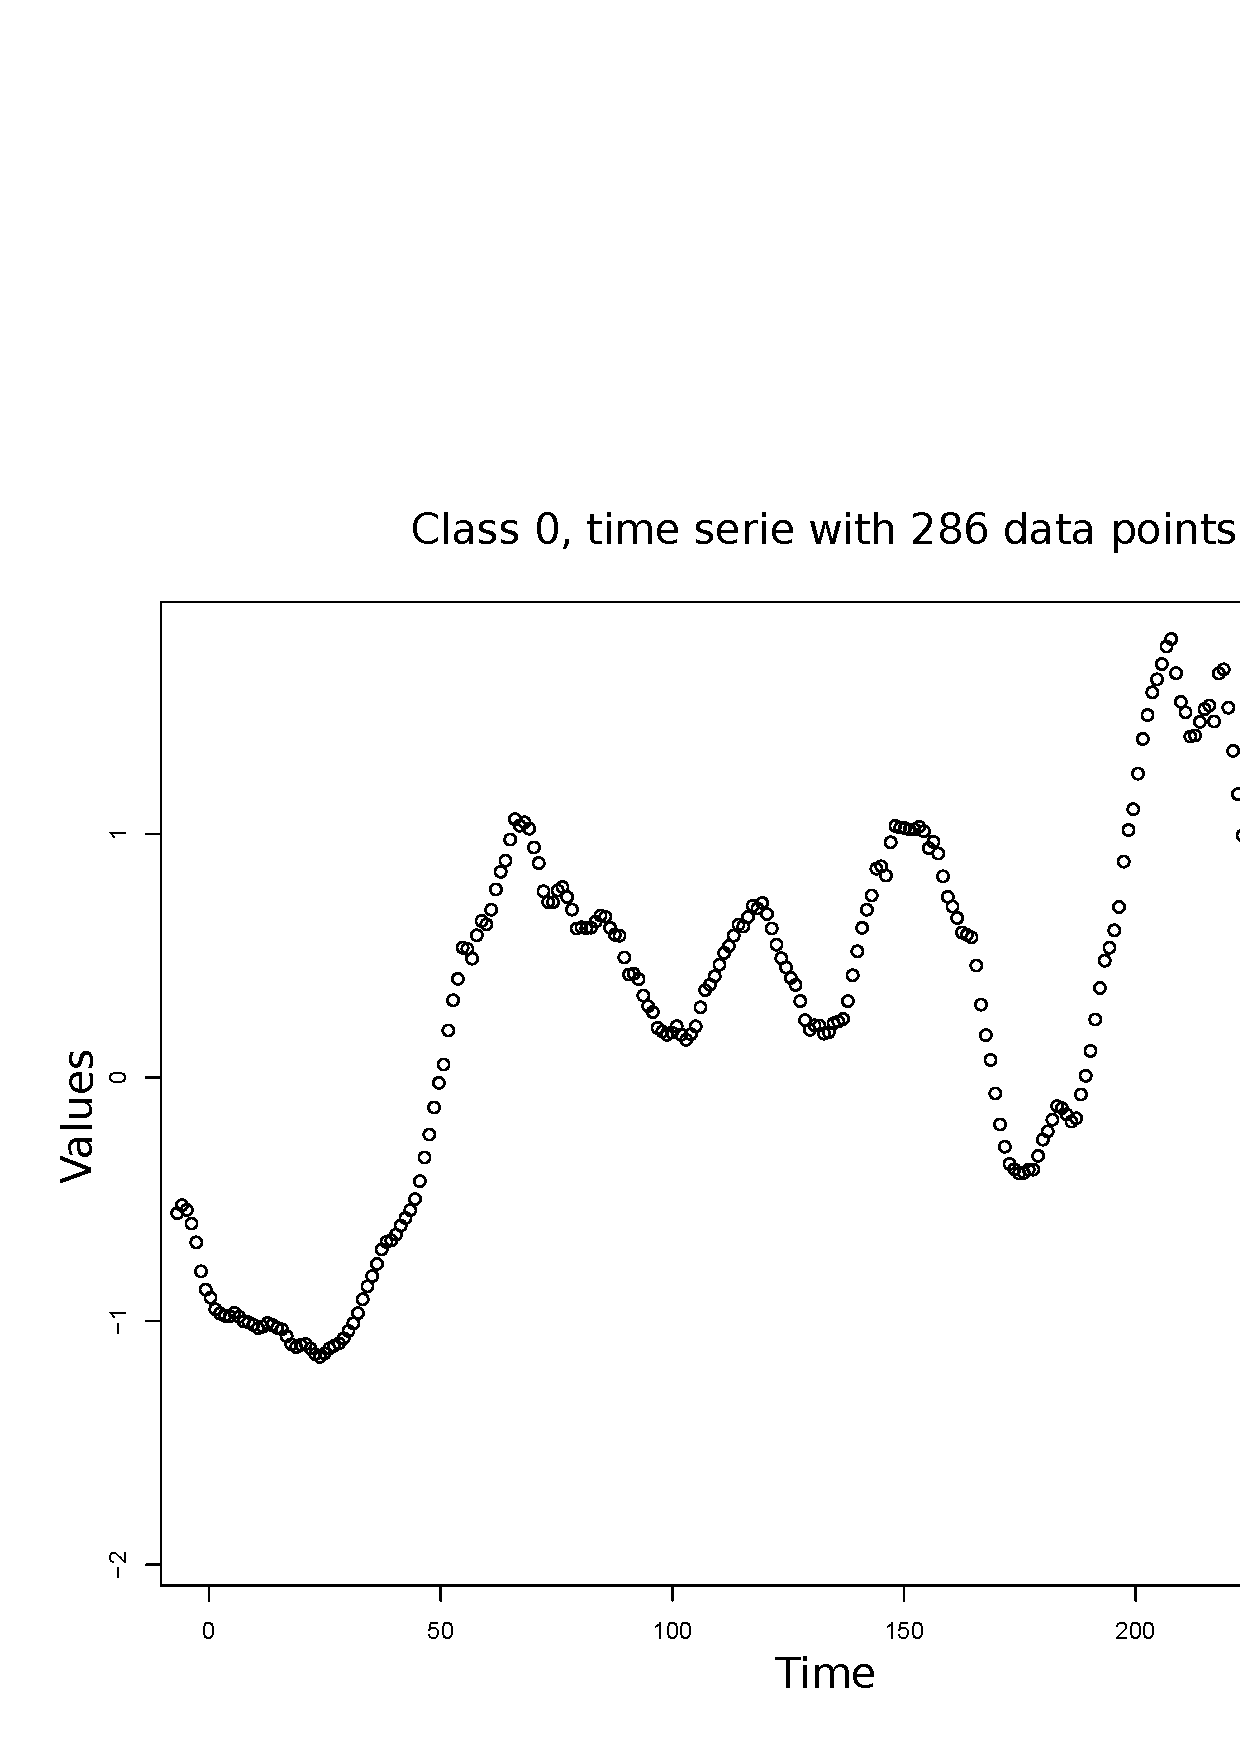
\includegraphics[scale=0.18]{images/coffee_0_ts}
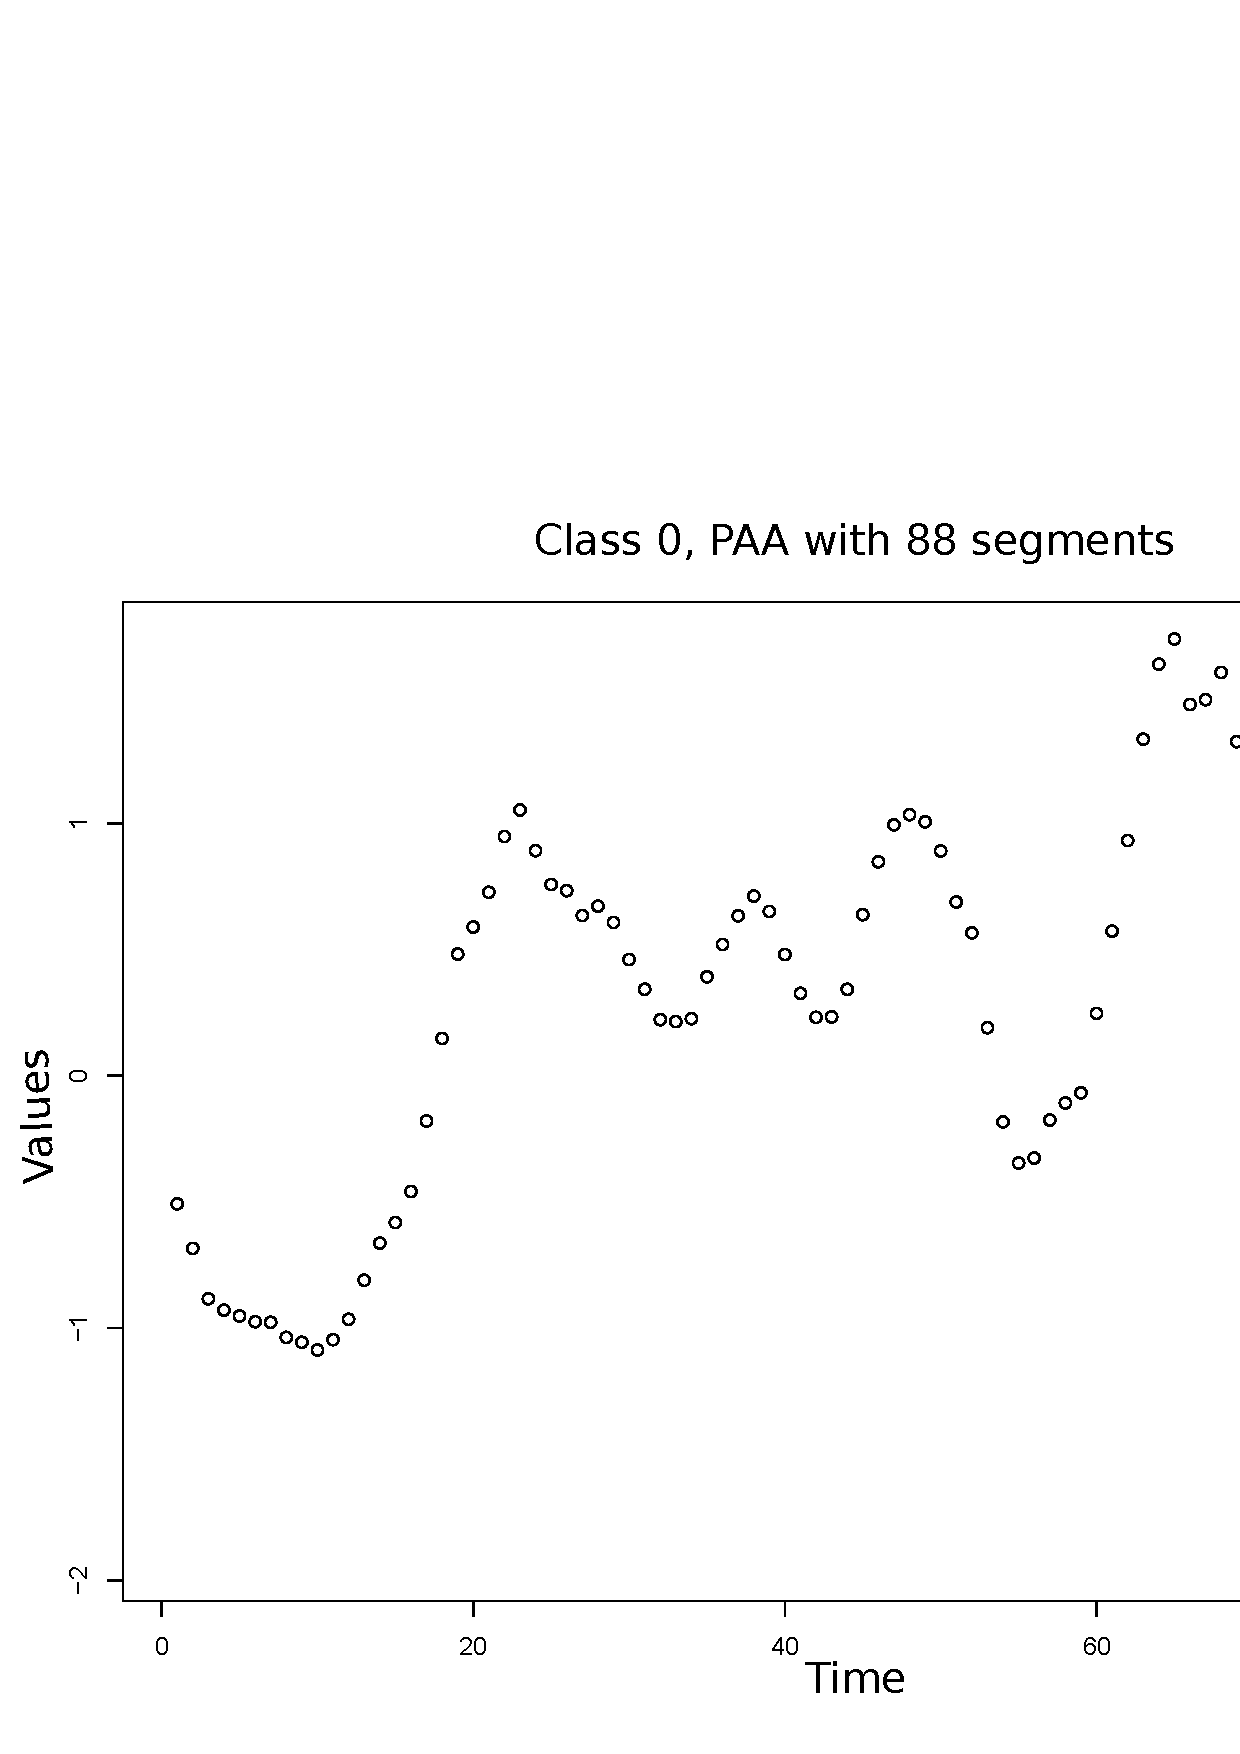
\includegraphics[scale=0.18]{images/coffee_0_paa_88}

%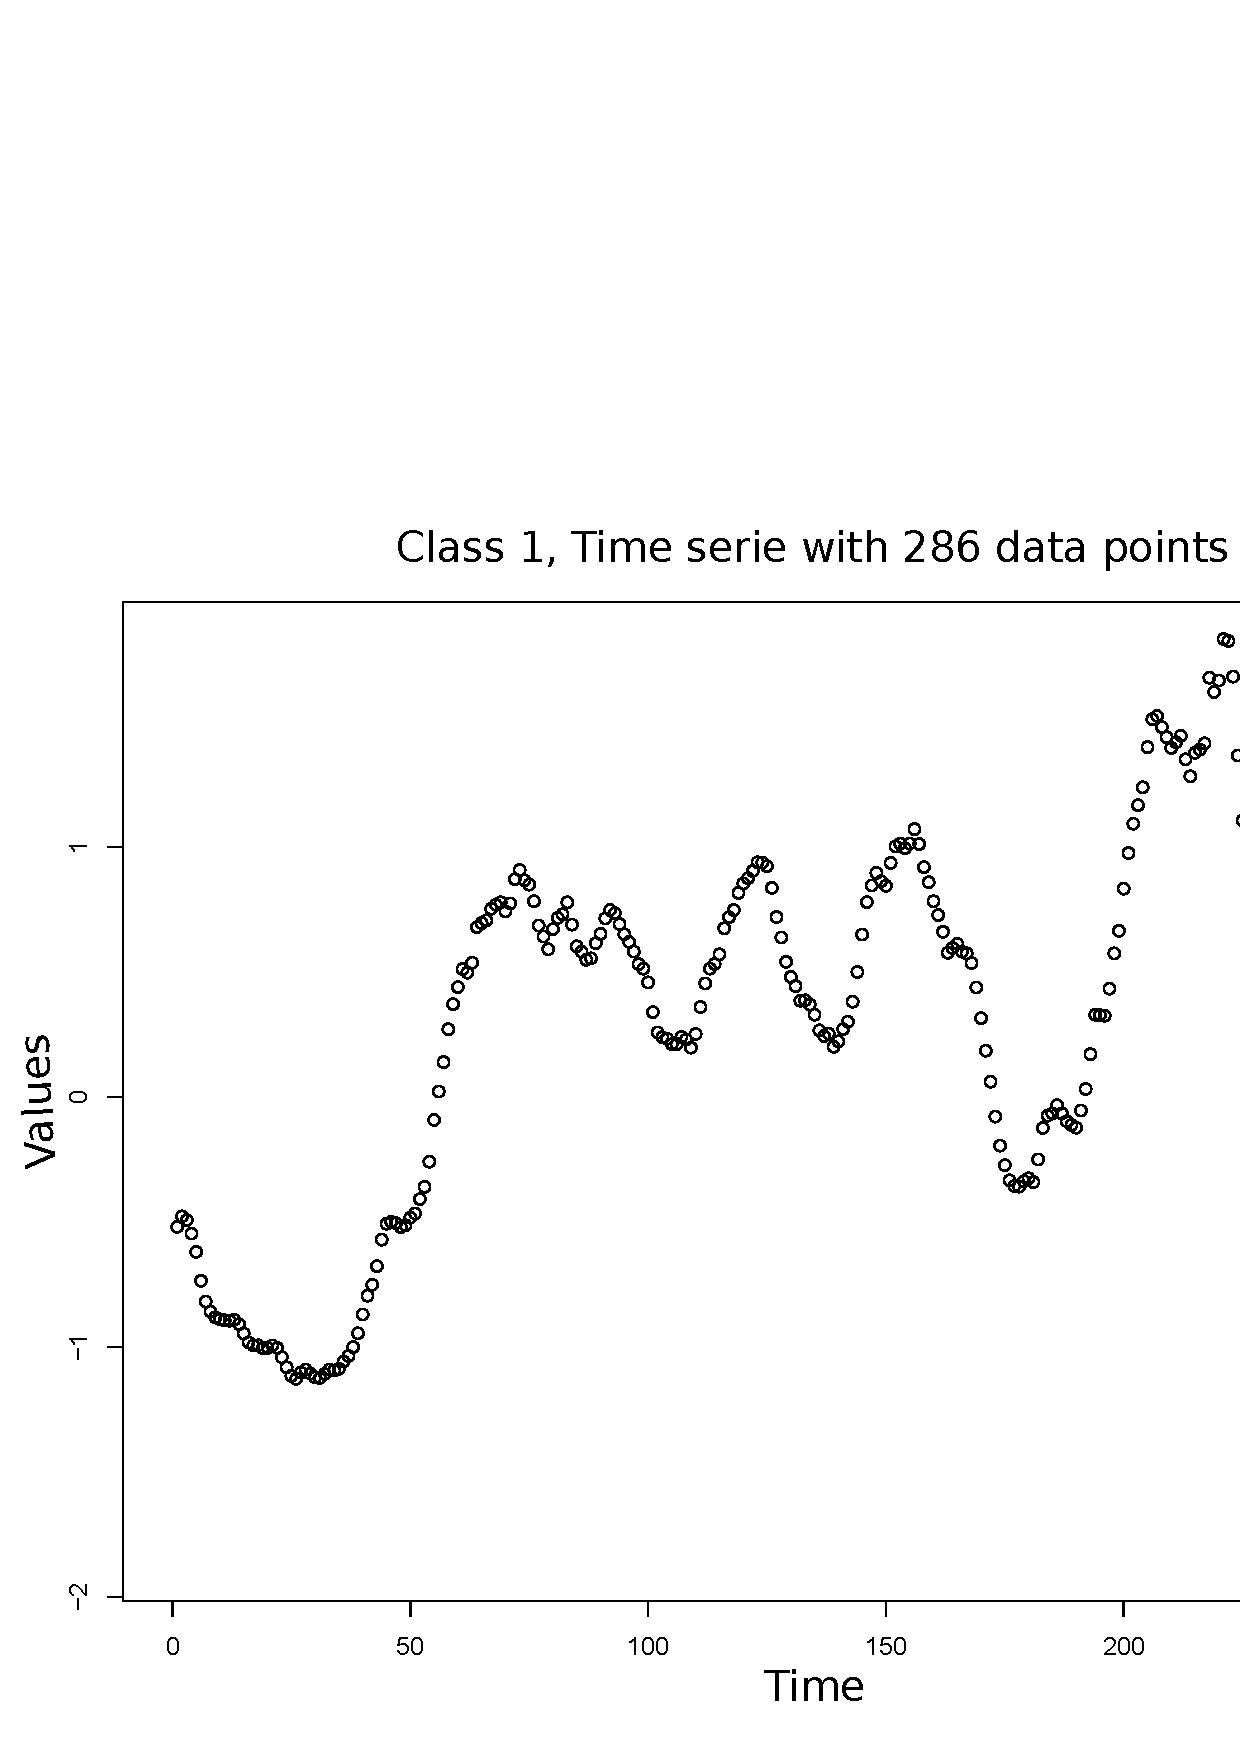
\includegraphics[scale=0.21]{coffee_1_ts}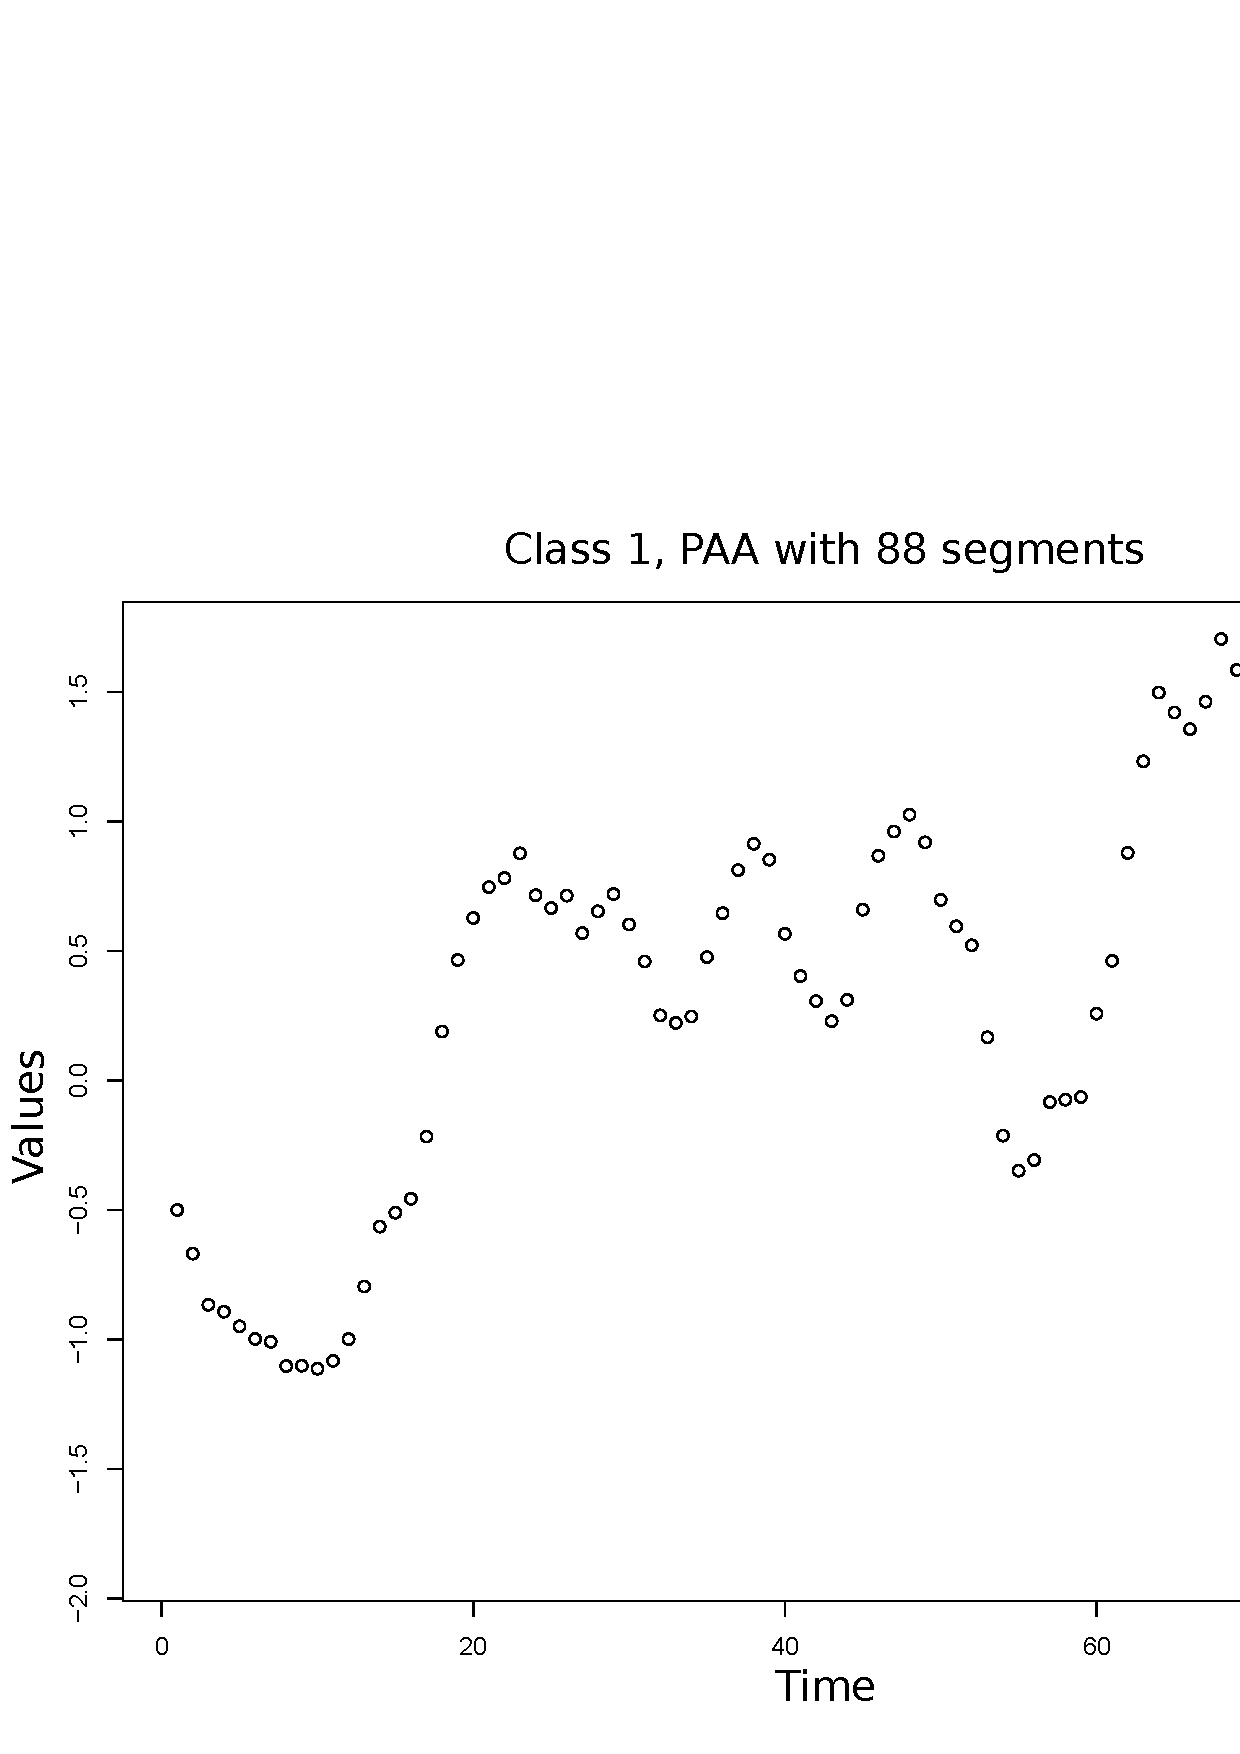
\includegraphics[scale=0.21]{coffee_1_paa_88}

\caption{Coffee dataset time series compression with PAA: original time series
(left) versus PAA represetion using 88 segments (right). The number of segments
is found by FDTW and allow to reduce the length of the time series while retaining the information that it contains.}

\label{coffee}
\end{figure}



\subsection{Classification}
To evaluate the quality of FDTW, we compared its classification errors with that of 35 other classification algorithms \cite{bagnall2016great} of the literature on 84 datasets of UCR archive{{}}.
The classification error  was calculated  based on the holdout model evaluation. FDTW used
the training set to find the number of segments $N$ using 3-fold cross-validation. If two
numbers of segments $N_1$ and $N_2$ are associated with the same classification error, we retain the
largest. The performances of the algorithms are compared using 
the Nemenyi test that compares all the algorithms pairwise and  provides an intuitive way to
visualize the results (Fig. \ref{cd2}). The Nemenyi test allows ranking the classification algorithms according to their average accuracy on 84 datasets.


The value of the segment number N found on the training set may in some cases not be appropriate for the testing set. We speak of an error of generalization which is due to the representativeness of the training set. Thus, FDTW obtains good results on the simulated data sets 3rd / 37 algorithms in terms of average accuracy (Fig. \ref{cd2}) because the data of the training set and the testing set are generated by the same models.

\begin{figure}
\centering
\includegraphics[scale=0.23]{images/cd1}
\caption{Critical difference diagram for FDTW and $36$ other classification algorithms on 6 simulated datasets.}

\label{cd2}
\end{figure}



However, to evaluate the significance of the difference between the classification algorithms on 84 datasets, we use the Wilcoxon signed rank test with continuity correction which has more statistical power.The results of these experiments are summarized below. 

The experiments show that despite data compression : 
\begin{itemize}
  \item  FDTW have better performance than Naive Bayes (NB), C45,  logistic regression (Logistic), BN;
  \item FDTW has similar performance to that of 26 other algorithms in the literature, namely : SVMQ, RANDF, ROTF, MLP, EUCLIDEAN\_1\_NN, DDTW\_R1\_1NN, DDTW\_RN\_1NN, ERP\_1NN, LCSS\_1NN, MSM\_1NN, TWE\_1NN, WDDTW\_1NN, WDTW\_1NN, DD\_DTW, DTD\_C, LS, BOP, SAXVSM, TSF, TSBF, LPS, PS, CID\_DTW, SVML, FS, ACF;
  \item DTW\_F, Shapelet Transform (ST), BOSS, Elastic Ensemble (EE) and COTE perform better overall than FDTW.
\end{itemize}

This demonstrates its competitiveness. Moreover, FDTW
outperforms the best result reported in the literature on  UWaveGestureLibraryAll dataset (Fig.
\ref{geste}).
The challenge with the UWaveGestureLibraryAll dataset is to recognize the gesture made by a user
from measurements made by accelerometers. As reported here \cite{Bagnall} the best accuracy obtained
on this dataset is 83.44\% with TSBF algorithm. FDTW outperforms this result and allows to obtain \textbf{91.87\%} of accuracy.


\begin{figure}[h]
\center
\includegraphics[scale=0.1]{images/c1}
\includegraphics[scale=0.1]{images/c2}
\includegraphics[scale=0.1]{images/c3}
\includegraphics[scale=0.1]{images/c4}
\includegraphics[scale=0.1]{images/c5}
\includegraphics[scale=0.1]{images/c6}
\includegraphics[scale=0.1]{images/c7}
\includegraphics[scale=0.1]{images/c8}

\caption{Eight types of time series corresponding to the vocabulary of 8 gestures.}

\label{geste}
\end{figure}



\section{Conclusion}
\label{sec:4}
Our problem in this paper was to choose an appropriate number of segments to compress time series with PAA in order to improve the alignment with DTW. To achieve this goal we proposed a parameter Free heuristic named FDTW with approximate the optimal number of segment to use. The experiments show that our heuristic increased the quality of alignment of time series with especially on synthetic datasets where DTW associated with PAA perform better than any other variant of DTW on a classification task and was rank 3/37 behind two ensemble classification algorithms COTE and EE. This work allows reducing the storage space and the processing time of time series while increasing the quality of the alignment of DTW. 
The same strategy presented in FDTW can be used to find the number of segments to be considered for the indexation and for symbolic representations of time series like SAX \cite{lin2003symbolic}, ESAX \cite{lkhagva2006extended}, SAX-TD \cite{sun2014improvement}.
